\documentclass[12pt, a4paper]{article}

% Packages used
\usepackage{authblk}
\usepackage[margin=3cm]{geometry}
\usepackage{graphicx}
\usepackage{hyperref}
\usepackage{mathpazo}

\parindent 0mm
\parskip 2mm

% Meta
\title{CRSU Startup Procedures}
\author{Michal~Rigan, Martti~Nirkko}
\affil{University of Sussex}
\date{\today}

\begin{document}

% Title page
\maketitle
\begin{abstract}
	This document details the startup procedures for the SNO+ remote control room at Sussex (CRSU). The basic setup, requirements and procedures to follow when starting up the control room and ideas for improvement are discussed. For a more detailed description of the setup, please refer to the CRSU commissioning report (\href{https://www.snolab.ca/snoplus/private/DocDB/cgi/ShowDocument?docid=5063}{DocDB-5063}).
\end{abstract}
\vspace{2cm}

\begin{figure}[htp]
	\centering
	
\includegraphics[width=0.8\textwidth]{../Miscellaneous/crsu_mascot}
	\caption{The correct prononciation of ``CRSU'', and its adorable mascot.}
	\label{crsu_mascot}
\end{figure}
\clearpage

% Table of contents (not required for a <10 page document)
% \tableofcontents
% \clearpage

% Main matter
% -----------
\section{Basic setup}
Machines abbreviations:
\begin{itemize}
	\item Operating machine (Mac) = \textbf{\tt opersu}
	\item Monitoring machine 1 (CentOS) = \textbf{\tt monsu1}
	\item Monitoring machine 2 (CentOS) = \textbf{\tt monsu2}
\end{itemize}

\begin{figure}[htp]
	\centering
	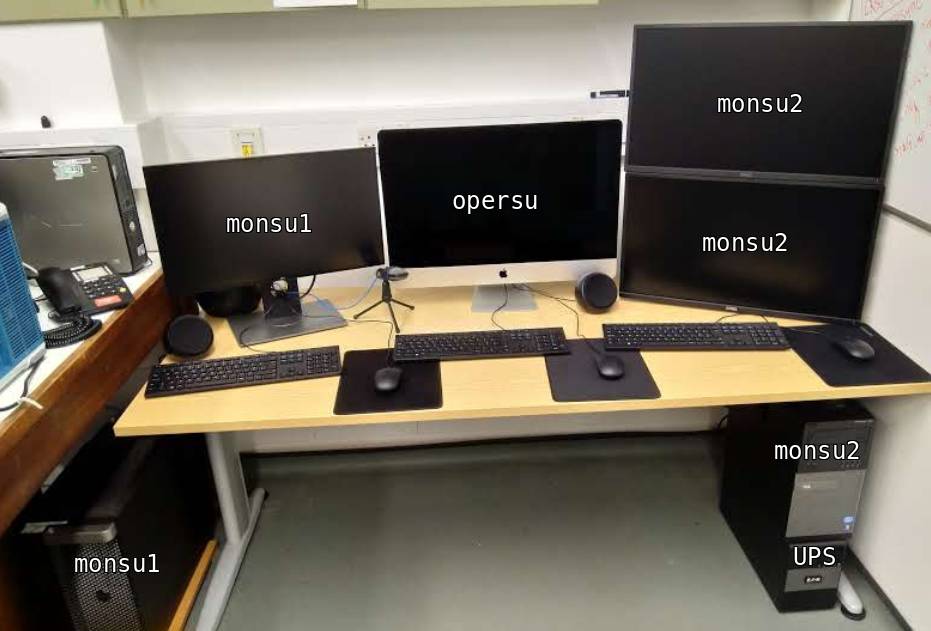
\includegraphics[width=\textwidth]{images/CRSU_final}
	\caption{The SNO+ remote control room at Sussex (CRSU).}
	\label{crsu_setup}
\end{figure}

Figure~\ref{crsu_setup} shows the current setup at CRSU: {\tt monsu1} is the machine on the bottom left, connected to the very left monitor and the left pair of peripherals. {\tt opersu} is the central machine, with the machine in-built into the monitor, connected to the central pair of peripherals. {\tt monsu2} is on the right, with the double display setup. The power buttons are on the top left of both {\tt monsu} machines and on the bottom left (backside) of the operating machine. Note that {\tt monsu1} can take longer time to boot-up due to the RAID system and dual boot setup. {\tt monsu2} sometimes warns about incorrect date settings on startup, just press F1 whenever you see the warning message. In addition, there is Windows running on a Virtual Machine (VM) on {\tt monsu1} and the process is described below. Every device except the landline telephone (which is powered by an ethernet socket alone) is connected to an Uninterruptible Power Supply (UPS) at the bottom right, below {\tt monsu2}.

All machines have the 2 usual accounts configured: the {\tt snoperator} and the {\tt snotdaq} account. For {\tt monsu} machines, you need to enter the account name at login as well ({\tt snoperator}). Additionally, {\tt root} acounts are available on the {\tt monsu} machines. Martti's staff account has admin rights on {\tt opersu}. Contact the remote control room experts
\begin{itemize}
\item \href{mailto:M.Nirkko@sussex.ac.uk}{M.Nirkko@sussex.ac.uk} / @mnirkko / {\tt +44 7948 759 907}
\item \href{mailto:M.Rigan@sussex.ac.uk}{M.Rigan@sussex.ac.uk} / @MichalR / {\tt +44 7467 380 455}
\item \href{mailto:Charlie.Mills@sussex.ac.uk}{Charlie.Mills@sussex.ac.uk} / @Charlie Mills / {\tt +44 7794 767 401}
\end{itemize}
if you require details or run into trouble.

% -----------
\section{Requirements}
This list notes the essential requirements needed to access the remote control room:
\begin{itemize}
	\item SALTO access card: this is a card that allows people to access the Pevensey II. It is needed to get to the building outside the normal working hours (especially important for graveyard shifts!). Speak to Simon Peeters: \\\href{mailto:S.J.M.Peeters@sussex.ac.uk}{S.J.M.Peeters@sussex.ac.uk} / @sjmpeeters / {\tt +44 7771 907 291}.
	\item Access to the remote control room (``InvisiblesLab'', office 4A23 on 1st floor of Pevensey II building) is code restricted.  Speak to Simon Peeters to gain access.
	\item Your SNOLAB account details to log in to the VPN software.
	\item The {\tt snoperator} password and the global collaboration log in details.
\end{itemize}

% -----------
\section{Long term shutdowns (10 or more days)}
Before a detector shift is taken at a remote shift station, the shifter must make sure that all the software is up to date on the operator and monitoring machines. This not a problem unique to remote stations - the software on site machines also has to be properly maintained - but there is a frequency of use difference. If a remote station has not been used for 10 or more days the following checklist should be completed. All checks and tests should be run the day before the scheduled shift.

\begin{figure}[htp]
	\centering
	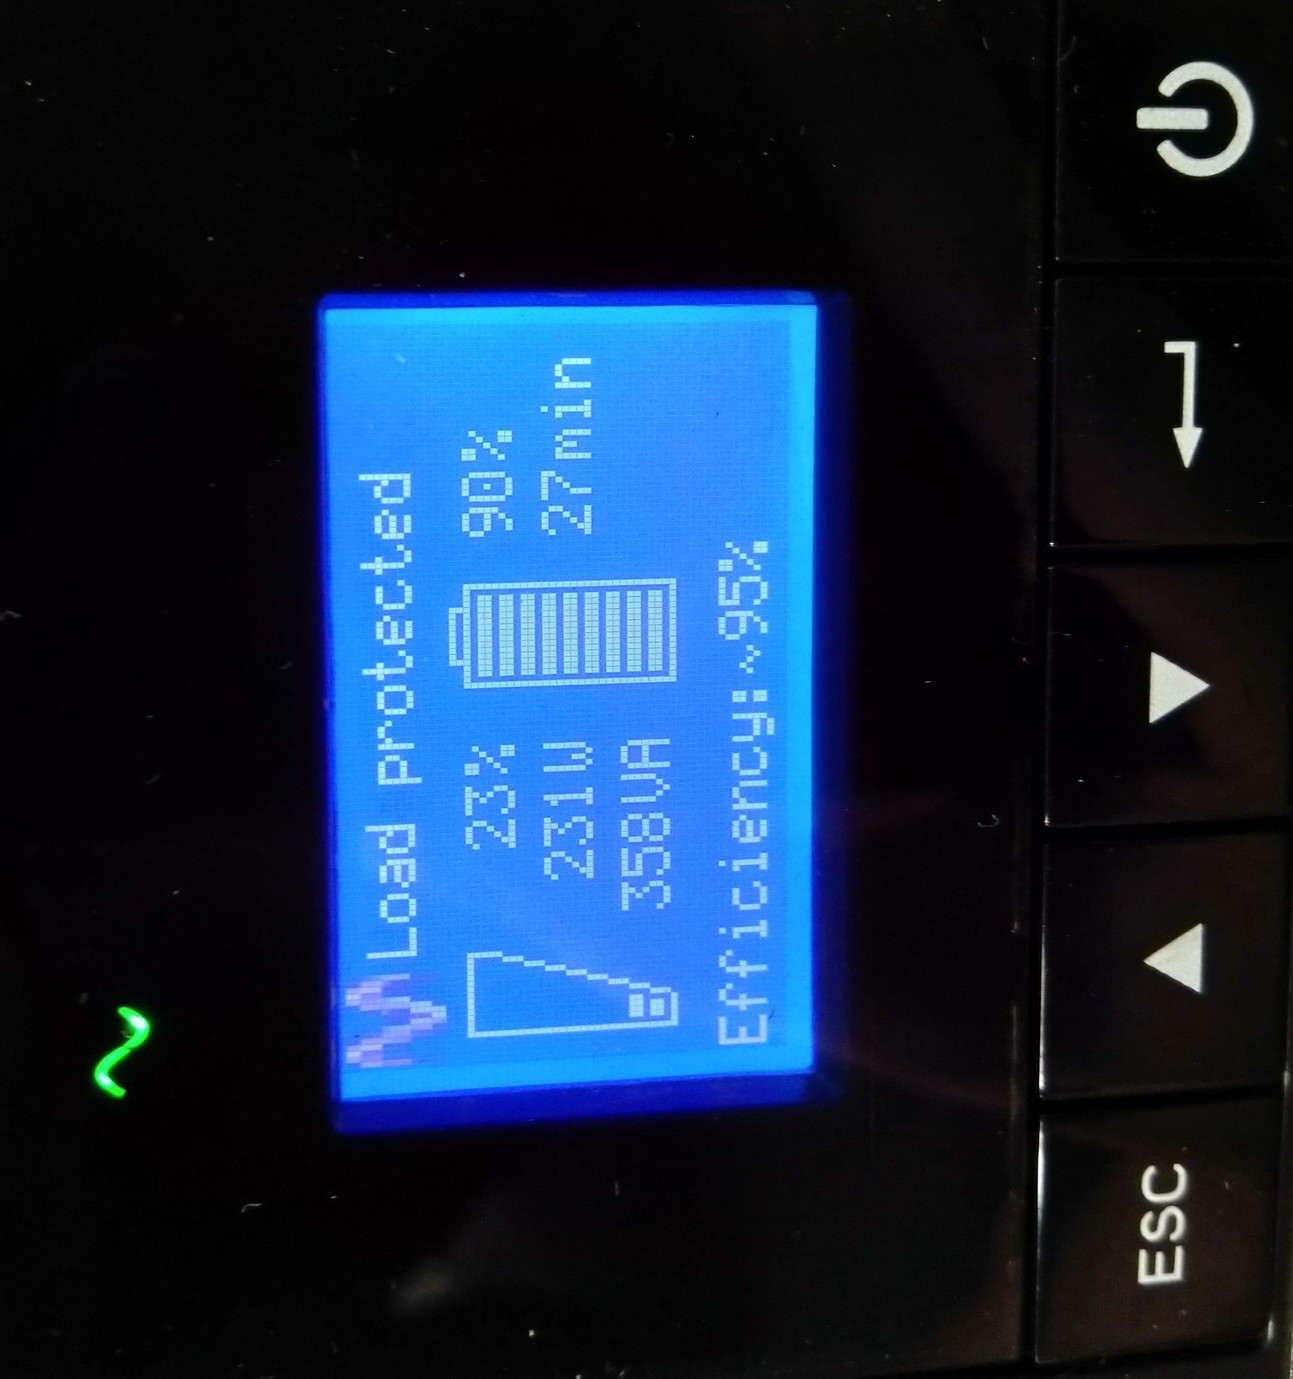
\includegraphics[angle=270,width=0.6\textwidth]{images/UPS_display}
	\caption{Display on the UPS, indicating current load.}
	\label{ups_display}
\end{figure}

\begin{itemize}
	\item \textbf{Power on UPS}: First, turn on the wall power on the far right, behind the {\tt monsu2} monitors. Then, turn on the UPS by pressing the power button for 2 seconds. It will make some noise as it turns on, the fan will be clearly audible. The display should indicate the current load and remaining battery time in case of a power outage, as seen in Figure~\ref{ups_display}.
	\item \textbf{Restart all machines}: this clears out the cache and temp files, frees up RAM, kills unwanted services and (possibly) allows updates to be installed.
	\item \textbf{Log in} as {\tt snoperator} on all machines!
	\item \textbf{Start the VPN}: this needs to be done on all machines. Find ``Cisco AnyConnect VPN'' (icon on the {\tt opersu} apps dock (bottom of the screen) and monsu apps bar (top left)). Use your SNOLAB IT account and log into {\tt SL-SNOPLUS} for {\tt opersu} and {\tt monsu} and {\tt SL-GEN} on Windows VM. Select ``Connect Anyway'' if there is a pop-up.
	\item \textbf{Check for updates}:
	\begin{itemize}
		\item Linux: System tab $\rightarrow$ Administration $\rightarrow$ Software Update \\
		      (you can also use the aliases {\tt update} and {\tt update-linux})
		\item Mac: On {\tt opersu}, click the Apple symbol in the application bar \\
		      $\rightarrow$ About This Mac $\rightarrow$ Software Update 
		\item Windows: In the VM on {\tt monsu1}, check if there are updates available using the window update icon in the bottom-right corners (there are none available if it is not there).
	\end{itemize}
\end{itemize}

% -----------
\section{Startup procedures}
The usual procedure to start up all required software (note that the {\tt monsu} machines have multiple virtual workspaces that you can navigate around using the CTRL + ALT + Arrows) is as follows:
\begin{itemize}
	\item {\bf Double-check that the wall socket is switched on!} Then power on the UPS and the physical machines, and log in as {\tt snoperator}. 
	\item Start-up Windows on the VirtualBox: On {\tt monsu1} there is an icon ``Oracle VM VirtualBox'' located on the top right of the desktop. Start the app, select the latest snapshot of Windows 7 Pro (either double click the item in the list on the left or click the ``Start'' green arrow). Log in as snoperator. Connect to VPN using the ``VPN Client'' icon on the desktop. Connect to the {\tt SL-GEN} group. (Connecting to the VPN on Virtual machine can result in disconnecting from another VPN on another machine - this is Cisco security to prevent from overloading. Be sure to reconnect and everything runs fine - it only disconnects once!). Start up the phone application by selecting the ``IP Phone'' icon on the desktop. %Finally open the UPS platform\footnote{Note that this refers to the detector UPS located at SNOLAB, not the one powering this remote shift station.} using the bookmark in firefox web browser (the UPS platform only works on {\tt SL-GEN}, therefore can only be opened on this VM).
	\item Connect to VPN software on all machines: Find ``Cisco AnyConnect VPN'' (icon on the {\tt opersu} apps dock (bottom of the screen) and monsu apps bar (top left)). Use your snolab account and log into {\tt SL-SNOPLUS}. Select ``Connect Anyway'' if there is a pop-up (again, check if you weren't disconnected randomly on other machines)
	\item On {\tt monsu1}:
	\begin{itemize}
		\item Start up: Alarm GUI, FEC FIFO, MTC GUI, Supernova monitor, DAQ log, Builder log and Deck GUI by clicking appropriate icons on the desktop (use multiple workspaces as appropriate). Sometimes a DB connection pop-up appears for the {\tt alarmGUI} (possibly other apps), use the collaboration log-in to connect. Supernova and Builder require the snoperator's password to connect.		
			\item Run Scope from the desktop (icon).
			\item This machine also runs Check Rates and Polling GUI when needed during the shift by selecting appropriate application on the desktop. List of all application is also available at Applications $\rightarrow$ Other from the taskbar.
		\item Make sure the virtual phone software is running on windows virtual machine as described above.
	\end{itemize}
	\item On {\tt monsu2} (this machine is dedicated to run high-load streaming apps):
	\begin{itemize}
		\item Run the local Dispatcher by clicking the icon on the desktop
		\item Start 4 copies of {\tt xsnoed} by clicking the icons on the desktop. There are specific icons to open Top or Bottom view {\tt xsnoed}, each of which will open the application on the respective monitor. The suggested settings are: live, sum (-PED), 100 NHit and 500 NHit environments (again, use as many workspaces as you like)
		\item Open the Minard stream in browser (bookmarks provided)
		\item Be sure to have Slow Control, Detector State, Detector State Check, Nearline Monitor, PMT Calibration Summary, Grafana (data-flow) and the Weather forecast (blizzards/thunderstorms) tabs open in a browser (bookmarks provided).
	\end{itemize}
	\item On {\tt opersu}:
	\begin{itemize}
		\item Connect to remote drive with orca files: ``Go'' tab from the taskbar (top left) $\rightarrow$ Connect to Server. Select {\tt buffer1} from the Favorite Servers
		\item Start TUBii audio by clicking the ``{\tt TUB\_audio.m3u}'' icon on the desktop. Be sure to disable video to decrease the load (Video $\rightarrow$ Video Track $\rightarrow$ Disable)
		\item When you are ready for the shift handover (having called the current shifter), right-click the {\tt snot\_main.Orca} file and select ``Open With'' $\rightarrow$ {\tt Orca (default)}. This ensures the correct version of Orca is opened instead of using the icon in the App doc
		\item Check correct version of Orca is running in \href{https://snopl.us/monitoring/orca-session-logs}{Orca Session Log}: Monitoring $\rightarrow$ Control Rooms $\rightarrow$ Orca.
	\end{itemize}
\item Be sure to have shift report page and Slack open at any of the machines (dedicated app installed at Mac)
\item To call international numbers (such as on-call expert), a number of prefixes are needed: dial {\tt 9-1470-00-number}.
\end{itemize}

% -----------
\section{Fire alarms}
In case of a fire alarm that lasts longer than 10 seconds, you will have to leave the building immediately. {\bf Stay safe} -- never risk personal harm! Make sure you have your mobile phone (with Slack installed!) and a piece of paper with the expert's contact details. If you incur a large personal phone bill due to an emergency handover, please claim this on staff expenses (budget code {\tt TB006-23}) and get Simon Peeters to sign it off for you.

% -----------
\section{Ideas}
\begin{itemize}
	\item Global SALTO card for lab?
	\item Improve fire alarm procedure.
\end{itemize}

% -----------
\end{document}
